\documentclass[conference]{IEEEtran}
\usepackage{times}

% numbers option provides compact numerical references in the text. 
\usepackage[numbers]{natbib}
\usepackage{multicol}
\usepackage[bookmarks=true]{hyperref}


\usepackage{amsfonts}                                                           
\usepackage{amsmath}                                                            
\usepackage{amssymb}                                                            
\usepackage{graphicx}                                                           
\usepackage{graphics}                                                           
\usepackage{epsfig}                                                             
\usepackage{mathptmx}                                                           
\usepackage{url}                                                                
\usepackage[l]{floatflt}                                                        
\usepackage{rotating}                                                           
\usepackage{subfigure}                                                          
\usepackage{multicol}                                                           
\usepackage{algorithm}                                                          
\usepackage{algorithmic}                                                        
\usepackage{verbatim}                                                           
\usepackage{listings}                                                           
\usepackage{chngpage}                                                           


\DeclareMathAlphabet{\mathcal}{OMS}{cmsy}{m}{n}

\renewcommand{\algorithmicrequire}{\textbf{Input:}}
\renewcommand{\algorithmicensure}{\textbf{Output:}}

\long\def\commentl#1{{\bf **Shih-Yun: #1**}}
\long\def\commentp#1{{\bf **Peter: #1**}}

\begin{document}

\title{Towards Modeling Real-world Human-robot Interaction that Prevents Overfitting}

\author{Paper-ID}

%\author{
%    \authorblockN{Shih-Yun Lo, and Peter Stone}
%    \authorblockA{
%        University of Texas at Austin\\
%        {\tt \{yunl;;pstone\}@cs.utexas.edu}
%    }
%}


\maketitle

%\begin{abstract}
%\commentl{TODO}
%\end{abstract}

\IEEEpeerreviewmaketitle

%%%%%%%%%%%%%%%%%%%%%%%%%%%%%%%%%%%%%%%%%%%%%%%%%%%%%%%%%%%
%%%%%%%%%%%%%%%%%%%%%%%%%%%%%%%%%%%%%%%%%%%%%%%%%%%%%%%%%%%
%%%%%%%%%%%%%%%%%%%%%%%%%%%%%%%%%%%%%%%%%%%%%%%%%%%%%%%%%%%

\section{Introduction}
\vspace{-0.3em}
\label{sec:intro}
\noindent
% [mobile robot navigation advances in dynamic environment]
In robotics, recent advances have allowed long-term autonomy for indoor mobile 
robot navigation, which has raised interest in the development of service 
robots that provide assistance to humans during daily activities. To achieve 
this objective, the robots need to be able to navigate smoothly among pedestrians, while 
not interfering with their ongoing activities. 
%This problem involves 
%modeling well the dynamics in human-robot interaction, where individuals have 
%independent goals to reach and potential collisions need to be avoided. 

% [human robot interaction scenarios]
Consider a robot navigating in a busy atrium with people walking towards 
different destinations. There is generally limited sensing of nearby agents, 
both by the human pedestrians and by the robot. It is not enough to reactively 
avoid imminent collisions. However, when predicting into the future, 
collision avoidance algorithms often fail to find a path in 
densely crowded environments, sometimes referred to as the "freezing robot 
problem"~\cite{trautman2010unfreezing}. For example, in human pedestrian 
navigation, it is commonly seen for agents to walk in front of one 
another to maximize their own travel efficiency, assuming other pedestrians 
are aware of the workspace occlusion and respond safely. Can the robot act 
the same way, while optimizing the joint efficiency of both agents?  

% [state of the art robot navigation in crowd]
To plan efficiently in dense crowds at the same time maintaining 
human-friendliness and safety, it is crucial to have good models of human 
responses to the robot's maneuvers. Many approaches have been proposed in the 
past decade to simulate human pedestrian dynamics~\cite{lamarche2004crowd, 
  treuille2006continuum, %paris2007pedestrian, 
karamouzas2009predictive}.
%Accordingly, robot planning in crowds has shown efficient performance in simulation
Look ahead planning, that includes a model of how others will react to one's 
own motion, is required. It's also important to keep in mind that people may 
respond to robots differently than they respond to other people. Large 
prediction errors of state-of-the-art approaches have suggested a large gap 
between real-world deployment and 
simulation~\cite{trautman2015robot,pfeiffer2016predicting}. When 
relying on models for lookahead planning, if people act unpredictably (or in a 
way not observed in the training data), safety can be compromised. 

%%to eliminate the gap between human-robot interaction modeling and real-world deployment
We therefore propose to train a predictive model from 
data collected during real-world human-robot interaction, and 
act online according to the learnt predictive model to obtain new training data. 
This iterative process will help ensure consistency between the robot's 
prediction of pedestrian's trajectories and their true trajectories in the 
presence of the robot's actual actions.

%With this process, we aim to achieve robot planning in 
%crowds that not only follows the inherent interaction patterns in human 
%pedestrians, but also counts in the noisy interaction where people intentional 
%block the robot.

%% to deal with human intentions for trajectory prediction
To achieve smooth robot maneuvering in human crowds, it is essential to 
systematically identify whether the person is focused on 
reaching their goal (conducting natural navigating behaviors), or may be 
distracted by the presence of robot (conducting unnatural navigating 
behaviors, such as blocking). To model this problem, we propose to first 
enable prediction of human traversal behaviors when encountering potential 
collisions, shown in Fig.~\ref{fig1}. 

%When the robot performs 
%``legibly''~\cite{dragan2013legibility} in those 
%situations, non-cooperative behaviors (intentional blocking) can be identified if not 
%classified into any type of traversal. 

 %we also propose to model the interactive dynamics based on local 
%observations, which helps the applicability of the approach in varied 
%environments. It is a contrained optimization problem on temporal collision 
%including its safety margins. The prediction process then falls in first deciding 
%which way the agent is prone to take, and how it would adapt its dynamics during 
%traversal. Accordingly, the controller looks ahead and optimizes the joint 
%efficiency subjected to the estimate of human traversal preferences.

We model the pedestrians as solving a constrained path optimization 
problem during traversal, which maintains the safe distances from the other agents while reaching 
their destination as quickly as possible. This approach provides us the 
capability to predict which path the 
pedestrian is prone to take to avoid, at what speed pattern. The robot can 
then optimize the joint efficiency by avoiding responsively to their 
preferences, ``legibly''~\cite{dragan2013legibility}, such that the pedestrian 
is clear about the robot's intention. A cooperative behavior is 
then expected on rational pedestrians, following the predicted traversal 
behaviors from our model; a non-cooperative behavior, like intentional blocking, can 
therefore be distinguished if not following any traversal patterns.

%Towards the deployment of a service robot in real world, the robust guarantee of safety during human robot interaction is important. Still, state-of-the-art modeling of this joint dynamics has limited capability when pedestrians engage in behaviors not presented in the training data. With complex model and unbalanced training data, the prediction model is under high risk of overfitting.

% local sensing, local representation (no global goal)
% the limited predicting capability when people engage in behaviors not present in the training data
%When navigating in a crowded environment, people observe other agents' behaviors, and act accordingly. With different dynamics observed, people conduct different motion patterns. The same situation applies to human robot interaction as well. If the pedestrians observe aggressive behaviors during robot navigation, they may perform conservatively by staying away from the robot to avoid collision; if the robot appears to be respond safely to disturbances in the environment, people may trust the robot more and interact with it more closely. 
%To solve this problem, we acknowledge that different pedestrian behaviors are excited under different robot maneuver policies. The learnt pedestrian dynamics may only capture partial interactive behaviors with the robot given its conducted policy. For example, if the robot navigates in the crowd with conservative avoiding behaviors, the learnt interaction would be limited as treated as a static obstacle; on the other hand, aggressive robot navigation may result in pedestrian avoiding behaviors where limited interaction is experienced. 

% introduce this work that does not overfit

\begin{figure}[tb]
  \begin{center}
  \hspace*{-1em}
  \subfigure[0.45\columnwidth][] {
    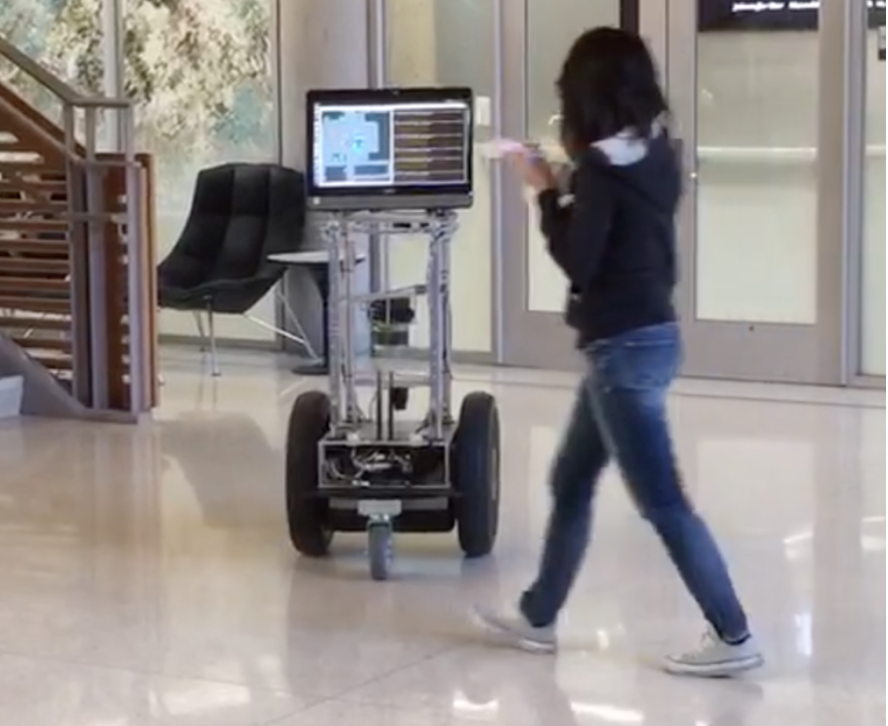
\includegraphics[width=0.5\columnwidth]{p1.png}
    \label{fig:p1}
  }\hspace*{-0.03em}
  \subfigure[0.45\columnwidth][] {
    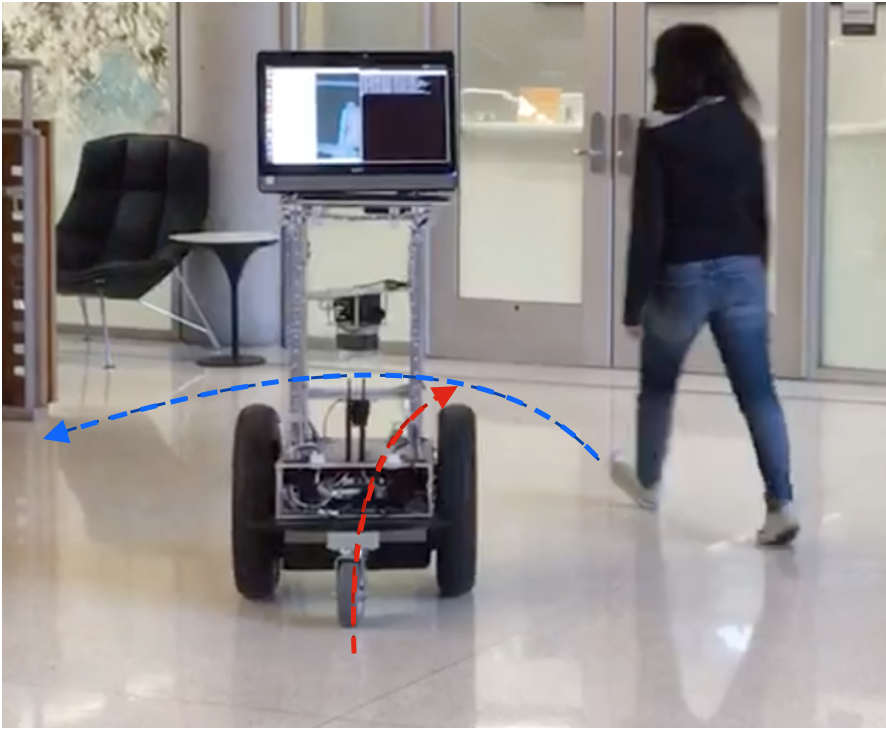
\includegraphics[width=0.5\columnwidth]{p2.png}
    \label{fig:p2}
  }
  \end{center}
  \vspace{-0.85em}
  \caption{The two pictures illustrate the common patterns of human 
    pedestrians passing the other agent (here the robot) to avoid a potential 
    collision (with the robot 
    moving towards the door, the pedestrian moving to the stair case at the left): {\bf (a)} to 
    decelerate and wait for the robot passing in front, 
    {\bf (b)} to accelerate and pass in front of the robot. Two styles of 
    traversal trade off between total path lengths and end speeds. While 
    slowing down to wait results in shorter paths, speeding up to pass in 
    front is also commonly observed when people navigate in crowds. 
    }  
  \vspace{-0.5em}
\label{fig1}
\end{figure}

\section{Related Work}
\label{sec:related}
\vspace{-0.4em}
% recent advance in crowd navigation modeling
% a) physics-based modeling of pedestrian spacing 
% b) inverse optimal planning techniques
The earliest attempt to model pedestrian behaviors was through a physics-based 
modeling approach, in which the spacing between pedestrians follows a 
potential field to generate collision-safe 
interactions~\cite{helbing1995social}. Following this work, explicit models 
for local collision avoidance were widely studied, to model the subtle 
adaptive personal-spacing behaviors in pedestrian 
interactions~\cite{papadakis2014adaptive}. Meanwhile, another community 
makes use of inverse optimal planning 
techniques~\cite{ziebart2009planning,henry2010learning,vasquez2014inverse} to 
model pedestrian dynamics by learning their policies assuming global observations and 
rational behaviors.

% a,b ignore the interactive dynamics in which one player's action affects the other's 
% c) joint decision making process
While the above approaches have shown to predict pedestrian motions 
offline or in simulation, an issue arose with the Markov Decision 
Process assumption when the methods were deployed on a robot to navigate in real world:
the real-time dynamics of pedestrians are also dependent on the robot's 
actions. 
%While the pedestrians treat the robot as an agent, they plan 
%accordingly to robot's motion. 

In this regard, a multi-player game setting including both human and robot actions into the joint state space was proposed in a Gaussian Process regression model and evaluated on a mobile robot in a fully-observed environment~\cite{trautman2010unfreezing}. This game setting has also shown significant results in autonomous cars through the consideration of human actions into their model to achieve communicative robot behaviors~\cite{sadigh2016planning}.

% d) prediction using offline training data does not always work: data may be from rational agents. Further, interactive data may only go from a small portion of state space, excited by pre-defined robot behavior 
Still, all of the above work are built from data collected by observing human-human 
interaction, which has degraded planning performance while encountering unmodeled 
human-robot interaction during real-world 
deployment~\cite{trautman2015robot, pfeiffer2016predicting}. To achieve 
cooperative interaction with humans and robots sharing a workspace, it is 
an essential capability for the robot to identify people's 
intentions, and then plan responsively to their actions. We propose to achieve 
better human-robot interaction in crowds by learning a predictive model 
iteratively through online interaction, and propose a predictive model 
that generates plans to avoid dynamic obstacles based on personal walking features. 
\section{Methodology}
We model the pedestrians as moving according to the solution to a constrained optimization 
problem, and formulate the constraints on the temporal collisions with 
(adaptive) safety margins, from a first person point of view. We assume that 
people have some fuzzy idea of the velocity of the other agent $v^o$, of their 
own velocity $v^p$, and the location where an expected collision will happen. 
The temporal constraint divides the 2D planning configuration space into two 
homotopy classes, which corresponds to two options of traversal decision, 
considering a two-player scenario: to slow down and traverse from behind by 
freeing the expected occupation at intersection (passive action, $a^{p}$, as 
shown in Fig.~\ref{fig:p1}), as well as to speed up and pass in front by postponing 
the expected intersection (active action, $a^a$ as shown in Fig.~\ref{fig:p2}).   

Note that, from the path planning perspective, there exists a third homotopy 
class to pass from behind by turning some degrees towards the other agent, 
resulting in earlier traversal time. This maneuver is not commonly seen in 
crowds simply 
because it results in a longer path and raises the risk of breaking into the 
other agent's safety margin. 

Based on the continuous control input $u^o$ (here the robot acceleration), the 
relative distance $d^{rel}$, and the adaptive safety margin $d^{saf}$ to 
allow for unexpected behaviors of the robot, we model the pedestrian 
decision making over passive ($a^p$) or active action ($a^a$) by logistic regression,
\begin{equation}
p(a=a^p|x,u^o) \sim \frac{1}{1+e^{w^Tf(x,u^o)}}, 
\end{equation}
where $x$ is the overall system state, including the pedestrian and confronting agent, and $f(x,u)$ is a feature function, capturing the relative dynamics of the two agents.

Preliminary results have suggested the dependency of people's traversal preferences 
on different regular walking patterns. For example, people who often traverse from 
the front, have a higher regular walking pace. Since the traversal 
behavior also depends on the robot's observed behaviors, we collect data under 
different robot navigation policies. In this workshop, we intend to show the 
robustness of the proposed pedestrian traversal decision predictor. We also 
intend to show the learnt interactive dynamics during traversal, through phase 
space analysis on velocity changes and positions. The resultant optimal 
policy that maximizes both agents' efficiency is expected to act legibly 
and responsively to the perceived human pedestrian traversal style. When the 
prediction fails and the risk of collision goes up, it is quite likely that 
the pedestrian is intentionally blocking the robot.
%The decisions of pedestrians are modeled on both waypoint selections (mixture model on different homotopy classes, based on speed, relative speed, spacing, and safety margins) and speed pattern adaptation (adaptive slow down or speed up to avoid collision, based on the same features). 

{\footnotesize
\bibliographystyle{plainnat}
\bibliography{reference}
}
\end{document}


